\problemname{Wiseguy}

\noindent Paulie Cicero is a made man who runs the underworld of Brooklyn along with his associates Jimmy ``the Gent" Conway, Tommy DeVito, and the young but ambitious Henry Hill. The crew just got wind of a one-in-a-lifetime opportunity to raid \$6 million from the Lufthansa vault at John F. Kennedy International Airport. If they plan carefully and succeed, this will go down as the greatest heist of all time.\\

Jimmy plans to hire $N$ new recruits for the operation, whom he plans to organize into a hierarchy of leadership. Recruits arrive one-by-one on a rolling basis. The first recruit has no leader, but every subsequent recruit that comes in must immediately be assigned to exactly one boss (who must be some previous recruit already in the hierarchy). Henry points out that for things to go smoothly, each recruit should in the end only be assigned 0, 1, or 2 subordinates -- either a left-hand man, or a right-hand man, or neither, or both. Setting a limit at 2 will reduce each individual's responsibility of having to manage lots of people.\\

Each recruit also has a distinct ``strength" level (say, measured as a distinct integer from $1$ to $N$), which Jimmy will evaluate and consider as he is assigning leadership. We can assume that the strength levels across all of the recruits are uniformly random, and that recruits arrive in no particular order of strengths. That is, the final sequence of strengths among the $N$ recruits ordered from oldest to newest is drawn uniformly randomly from the set of all $N!$ possible permutations.\\

Paulie knows from experience that having a strong recruit leading other weaker recruits is a bad idea (the boss might abuse the subordinates), as is having a weak recruit leading only stronger recruits (being more qualified than your boss can lead to insubordination). Henry came up with a simple rule to mitigate this problem and bring some balance: For each recruit $i$, the left-hand man (if he exists) should always be weaker than recruit $i$ himself. Conversely, the right-hand man (if he exists) should always be stronger than recruit $i$ himself.\\

Each new recruit that comes in is first handed to the first recruit (except the first recruit himself). Based on Henry's rule, the new recruit is passed down to become either the left- or right-hand man of the current recruit that has custody of him. If there is already a left- or right-hand man, then the recruit is passed down further. This repeats until there are no conflicts and the new recruit is settled in as a subordinate of an existing recruit who previously only had either 0 or 1 subordinates. The diagram below illustrates the boss assignment process for $N = 4$ recruits, who arrive in the following order of strengths: 3, 1, 4, 2.\\

\begin{center}
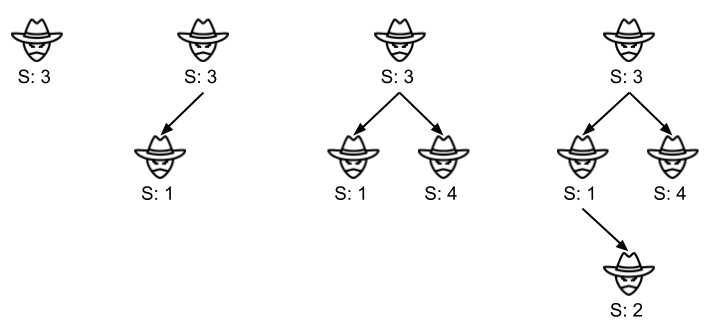
\includegraphics[width=300pt]{wiseguy}
\end{center}

While Henry's strategy of limiting the number of subordinates to 2 per person is good for distributing responsibility, the hierarchy can also become quite ``vertical". Having excessively long chains of command can lead to miscommunication and broken telephones, which the crew cannot afford in a delicate operation like this. The ``height" of a hierarchy is defined as the maximum number of times that a message needs to be passed from the first recruit to be able to reach any other recruit in the hierarchy. For example, the height of a hierarchy with a single leaderless recruit is 0, and the height of the last hierarchy in the above diagram is 2.\\

Given the uniform randomness of new recruit strengths as well as the rules above for assigning leaders, Henry needs your help in finding out the expected height of the final hierarchy. This can be thought of as the ``average" height of hierarchies across all possible arrival orders. For example, in the case of having to organize $N = 2$ recruits, both possible hierarchies have a height of 1. In the case of $N = 3$, two of the possible hierarchies have a height of 1, and the remaining four possible hierarchies have a height of 2, resulting in an expected height of $(1 + 1 + 2 + 2 + 2 + 2)/6 = 5/3 \approx 1.66667$.\\

Please help Henry predict the height for a hierarchy of $N$ recruits, so he can decide whether the plan will be feasible. A true wiseguy never gets caught, but a bad judgment or miscommunication in the ranks can easily bring shame to your crew. You'd better not mess up, or you might as well listen to Billy Batt's advice for Tommy -- quit the mob life, go home and get your shine box.\\

\section*{Input}
The first line of input consists of a single integer $T$ ($1 \leq T \leq 500$), specifying the number of test cases to follow.\\
$T$ lines follow, each of which is a test case consisting of a single integer $N$ ($1 \leq N \leq 500$), specifying the number of recruits that will need to be organized for the heist.\\

\section*{Output}
For each test case, print, on a separate line, a single real number denoting the expected height for the hierarchy.\\
Note: your answer must have at most $10^{-5}$ absolute or relative error to be considered correct.\\
